\chapter{実装}
\label{chap:implementation}

本章では、第\ref{chap:design}章で述べたプログラミング環境の構成要素について述べる。

\section{Babascript}

Babascriptは人への命令構文を持ったオブジェクトを宣言できるライブラリだ。
Node.js及びRubyで実装した。


\subsection{基本仕様}
人オブジェクトを宣言する

人オブジェクトに対するメッセージ送信によって、プログラム上にて人とコミュニケーションを取る

\subsection{人への命令構文}

人への命令構文を実行することによって、人への処理命令を送ることができる。
人オブジェクトを対象とし、命令内をそのままメソッドとして記述することによって人への命令構文として実行することができる。
人オブジェクトは、存在しないメソッドを全て人への命令構文として解釈する。
そのため、実装されていないメソッド名であれば、あらゆる命令をメソッドとして表現し実行することが可能である。
例えば、 \"toString\" などのメソッドは多くのオブジェクトに置いて定義されている。
このような、すでに定義されているメソッドは人への命令としては解釈されず、そのまま実行できる。
しかし、\"パスタを茹でる\"などのようなメソッドは定義は可能だが、実際に定義されているケースは非常に稀であると言える。
また、プログラム内で人オブジェクトに新たにメソッドを定義した場合なども、人への命令として解釈することはない。

\begin{figure}[htbp]
  \begin{center}
  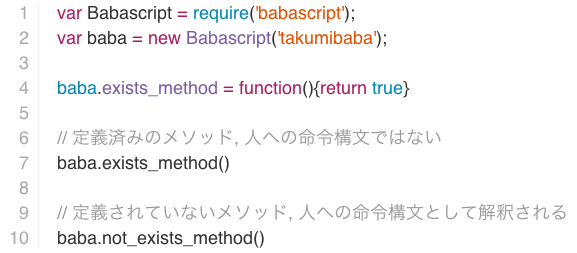
\includegraphics[width=.7\linewidth,bb=0 0 378 160]{images/methodmissing_sample.js.png}
  \end{center}
  \caption{人への命令構文}
  \label{fig:methodmissing_sample}
\end{figure}

オブジェクトに存在しないメソッドが呼び出された時に、特定のメソッドにその処理を委譲するような仕組みは、プログラミング言語Rubyなどにおいては
methodmissingなどと呼ばれる。
このような仕組みを利用することで、より人への命令手法として自然なメソッド名の記述が可能となる。

この際、メソッド名と第一引数は命令の内容として、タスク化され、ワーカーに送信される。
第一引数はオプション情報として評価される。
また、第二引数は、命令に対して何かしらの値が返された時に実行される。

\subsection{オプション情報の付加}

メソッド名以外に送信したい情報があるときには、第一引数にオプション情報としてオブジェクトを与える。
クライアントアプリケーション側でオプション情報を得ることができるため、このオプション情報に応じて
ユーザに提示する画面を変更するといったことが可能である。

オプション情報の例としては、返り値の型情報や、タイムアウト時間などが考えられる。
オプション情報は図\ref{fig:babascript_option}のように記述する。
図\ref{fig:babascript_option}場合であれば、返り値の型はstringで、3分後までに返り値を得られなかった場合は、
人力処理を止め、第二引数で指定するコールバック関数を実行し、処理を続行させるといったことをオプション情報として記述している。

\begin{figure}[htbp]
  \begin{center}
  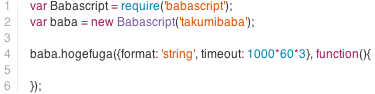
\includegraphics[width=.7\linewidth,bb=0 0 378 160]{images/babascript_option_sample.js.png}
  \end{center}
  \caption{オプション情報のサンプルソースコード}
  \label{fig:babascript_option}
\end{figure}

オプション情報である第一引数は省略可能である。
省略した場合は、自動的に図\ref{fig:option_default}のようなオブジェクトが代入される。

\begin{figure}[htbp]
  \begin{center}
  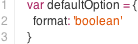
\includegraphics[width=.3\linewidth,bb=0 0 138 44]{images/option_default.js.png}
  \end{center}
  \caption{デフォルトのオプション情報}
  \label{fig:option_default}
\end{figure}


\subsection{コールバック関数}

命令構文の第二引数にコールバック関数を指定すると、実行結果を取得した後にこのコールバック関数が呼ばれる

人間は計算機の処理に比べて遅延しがちであるため、非同期を前提とした実装をしている

\subsection{タスク情報}

タスク情報は図\ref{fig:task_format}のように構成される。

\begin{figure}[htbp]
  \begin{center}
  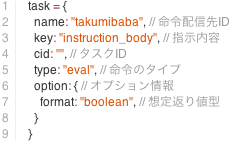
\includegraphics[width=.6\linewidth,bb=0 0 354 225]{images/task_format.js.png}
  \end{center}
  \caption{タスク情報}
  \label{fig:task_format}
\end{figure}

\section{Babascript Client}

Babascript Agent Applicationは、プログラムと人とのインタラクションを仲介する役割を持つ。

Javascript及びRubyで実装した。

機能としては、プログラムからの命令を受け取ることと、命令に対する人の処理結果を返すこと

Babascript Clientは、サービス部とインタフェース部から構成される。

\subsection{サービス}

命令の受け取りや返り値の送信などを担う

命令を受け取ると、イベントを発行する



\subsection{インタフェース}

ユーザとのインタラクションを行う。
命令をユーザに見せるのと、実際に実行結果を入力させる機能を持つ

例として、Webアプリケーションとして実装した。
% Android wear interaface and slack interaface のどちらか/双方が実装できたら
% 項目を増やして対応する。


\section{プラグイン機構}

Babascript 及びBabascriptClientはその機能を拡張するために、プラグイン機構を持つ。

以下の様に使うことで、Babascript及びBabascriptClientによってイベントが発生した時に、
それに応じたデータを受け取り、自由に操作することができる。

Babascript及びBabascriptClientは、以下のイベントを受け取る。

- initialize
- connect
- send
- receive

\subsection{具体例}



\subsubsection{Logger Plugin}

LoggerPluginは、

\subsubsection{Datasync Plugin}


% Adapter
\section{通信手法}

Babascript及びBabascript Clientは、通信手法を切り替えることが出来る
この通信モジュール部分をBabascript Adapterと呼ぶ。

% ここの区分、どうしよ?
% Node-lidaの利用は前提とする?
% Node-linda Socket.IO Adapter
% Node-linda Pushnotification Adapter
% こんな感じの分け方でいい気がする。
% 今はnode-lindaを利用してるけど、Adapterは非常に簡単に開発できる、みたいな。

\subsection{Node-Linda}

\subsection{Node-Linda Adapter}

Node-Linda Adapterは、Socket.IOを用いてNode-Lindaというプラットフォームに接続する。

構成図は以下のような感じになる。

\subsection{PushNotification Adapter}

Node-Linda Pushnotification Adapter は、HTTP RequestとPushnotificationを用いて
Node-Linda プラットフォームに接続する。
